\chapter{COMBAT SKILLS}

\begin{multicols}{2}

\index{Combat Skills}Combat skills determine which weaponry a character is able to wield, and in what specific way (if any) he can wield those weapons most effectively.

\section{COMBAT SKILL POINTS}

\index{Combat Skill Points}All characters are given Combat Skill Points at 1\textsuperscript{st} level, which they must immediately exchange for combat skills.  As initial combat skills represent years of training and practice prior to becoming 1\textsuperscript{st} level, those not exchanged during character creation are lost.  Additional Combat Skill Points (CSP) are earned at higher levels.  A character is considered to be unskilled in the use of a weapon or other combat skill, unless they exchange a combat skill point to become skilled.  Once a combat skill has been chosen, the decision is permanent.

\noindent
\begin{minipage}{\columnwidth}

\captionof{table}{Skill Points by Class}\label{classCSP}
\noindent
\begin{tabular}{|p{0.31\columnwidth}|p{0.36\columnwidth}|p{0.18\columnwidth}|}
\hline
Class		& Combat Skill Points	& Unskilled Penalty \\
\hline\hline
\rowcolor[gray]{.9}Warrior			& 4~+~1 per 3 levels	& $-2$/$-1$ \\
Priest or Rogue	& 2~+~1 per 4 levels	& $-3$/$-2$ \\
\rowcolor[gray]{.9}Wizard			& 1~+~1 per 6 levels	& $-5$/$-3$ \\
\hline
\end{tabular}

\end{minipage}

\paragraph{Class:} Each class group is represented.  Multi-classed characters use the most advantageous row for their respective classes, and do not add them together.  A fighter/mage simply uses the warrior row.  Note that priests and rogues have identical combat skill potential.

\paragraph{Combat Skill Points (CSP):} \index{Combat Skills!Combat Skill Points}The formulae in this column indicate how many CSP the character receives at 1\textsuperscript{st} level and the next divisible level that a character will receive one additional CSP.  For example, a fighter has 4 CSP at 1\textsuperscript{st} level and earns 1 additional CSP at 3\textsuperscript{rd} level, another at 6\textsuperscript{th} level, etc.  If the GM allows, a character's Intelligence---Languages Known score may be added (in whole or in part) to the number of CSPs received at 1\textsuperscript{st} level.

\paragraph{Unskilled Penalty:} \index{Combat Skills!Unskilled Penalties}The first number in this column indicates the penalty applied to the character's THACO when using a weapon with which he is completely unskilled.  For example, a mage who is unskilled with daggers suffers a $-5$ penalty to his THACO.  The number following the slash indicates the penalty applied if a character wields a weapon that he is not skilled with, but he is skilled with a weapon in the same weaponry group (See below).  For example, if the mage were to be skilled with a knife, he would only suffer a $-3$ penalty when wielding a dagger.

\section{AMBIDEXTERITY}

\index{Ambidexterity}In exchange for 1 CSP, any character can become ambidextrous, but only warriors and rogues may fight with a weapon in each hand.  

\paragraph{Ambidexterity:} An ambidextrous character suffers no penalty when using his non-dominant hand for any actions.  In combat, this reduces the penalty suffered to attacks with his non-dominant hand by 2 while fighting with two weapons.  This skill stacks with a character's dexterity---missile attack modifier (Refer to Two Weapon Fighting and Attacks with the Non-Dominant Hand).  This skill is not considered a part of any method, and unskilled penalties are, by default, already assumed elsewhere in the rules.

\section{WEAPONRY SKILLS}

\index{Combat Skills!Weaponry Skills}One or more CSPs are usually exchanged for skill with a single weapon, a grouping or even a type of weaponry, but they can also be exchanged to become skilled in certain specific combat expertise and methods.  A character can only become skilled with weapons and methods allowed to his class.  If a character becomes skilled in a group or type of weaponry, they are still unable to wield weaponry in that group or of that type that is not allowed to their class.

\paragraph{Single Weapon:} The character becomes skilled with a single weapon in exchange for 1 CSP and totally negates the unskilled penalty associated with that weapon and partially negates the penalties for related weapons (Refer to Unskilled Penalty). 

\paragraph{Weaponry Group:} \index{Weaponry Groups}A weaponry group consists of weapons of similar design such as swords or pole arms.  By exchanging 2 CSPs to become skilled with a weaponry group, a character becomes skilled in all weapons within that group that are allowed to his class.  When adding new weapons to his world, the GM should consider which, if any, weaponry group that the new weapon belongs.

Note that the arquebus, blowgun and quarterstaff do not belong to any group and must be learned separately.

\noindent
\begin{minipage}{\columnwidth}

\captionof{table}{Weaponry Groups}\label{weapongroups}
\noindent
\begin{tabular}{|p{0.3\columnwidth}|p{0.6\columnwidth}|}
\hline
Group	& Weapons \\
\hline\hline
\rowcolor[gray]{.9}Axe				& Battle axe, hand/throwing axe, Pole axe (all) \\
Bow				& Bow (all) \\
\rowcolor[gray]{.9}Cavalry			& Flail, mace, pick (horseman varieties) \\
Club			& Club, morning star, war hammer \\
\rowcolor[gray]{.9}Crossbow		& Crossbow (all) \\
Infantry		& Flail, mace, pick (footman varieties) \\
\rowcolor[gray]{.9}Lance			& Lance (all) \\
Long blade		& Bastard sword, long sword, scimitar, two-handed sword \\
\rowcolor[gray]{.9}Medium blade	& Broad sword, cutlass, khopesh  \\
Short blade		& Dagger/dirk, knife, sickle, short sword \\
\rowcolor[gray]{.9}Pole arm		& Pole arm (all, including pole axes) \\
Release action	& Lasso, net, scourge, sling, staff sling, whip \\
\rowcolor[gray]{.9}Spear			& Harpoon, javelin, spear, trident \\
\hline
\end{tabular}

\end{minipage}

\index{Weaponry by Type}\paragraph{Weaponry By Type:} Weaponry types provide the character with the most diverse and widest selection.  They reflect those weapons that inflict the same type of damage, either by slashing (S), bludgeoning (B), or piercing (P).  By exchanging 3 CSPs, a character becomes skilled with every melee or hurled weapon of that type which is allowed to their class.  If a weapon inflicts multiple types of damage, it overlaps and is included under each type.  For example, many pole arms are included in both the piercing weaponry type along with short sword and the slashing weaponry type along with long sword (Refer to the Melee Weapon Table).  Non-lethal weaponry and ranged weaponry such as arquebus, blowgun, bow, crossbow are not included.

\section{COMBAT METHODS}

\index{Combat Methods}In addition to the option of weaponry specialization, single class fighters can choose to become skilled in any or all of the following combat methods but only one method may be chosen at 1\textsuperscript{st} level (the GM may make an exception in the case of Unarmed Combat Methods and single class fighters, q.v.).  Other warriors, rogues, priests and any multi-class combination can only become skilled in one combat method, ever.  Single class wizards can only ever become skilled in one of the ranged weaponry or unarmed combat methods.

In exchange for 1 CSP, a character becomes skilled in a method, granting bonuses when using weapon(s) which both meet the requirements of the method and in which he is skilled.  For example, a character skilled in the single-weapon method and with the cutlass but not the long sword gains bonuses for single-weapon method if fighting with a cutlass but not with a long sword (assuming all other conditions of the method have been met).

\index{Melee Weaponry Methods}\subsection{MELEE WEAPONRY METHODS}

There are four melee weaponry combat methods: single-weapon, two-handed, weapon-shield and dual-weapon.  Single class wizards may not exchange CSPs for melee weaponry methods.

\index{Single-weapon Method}\paragraph{Single-Weapon Method:} Often chosen by single class rogues, this method involves defending oneself while fighting with one weapon in the character's dominant hand.  No other weapons or shields can be used in a non-dominant hand although small items (such as a potion) may be held.  \index{Armor Class!Effects of Single-weapon Melee Weaponry Method}A character skilled in this method gains a $-1$ bonus to their AC.  When gaining additional CSP, the character may exchange a second one to gain specialization in this method, increasing the bonus to AC a maximum of $-2$.

\index{Two-handed Method}\paragraph{Two-Handed Method:} Useful whenever a character fights with one weapon in both hands.  Some weapons require both hands to use while others give the option of using both hands (in this case, the bonus is only applied when using them with both hands).  Character's skilled in this method reduce their two-handed weapon's combat speed by 3 (to a minimum of 0).

\index{Weapon/Shield Method}\paragraph{Weapon-Shield Method:} Preferred by many priests and warrior types and colloquially referred to as ``mace and board", ``sword and board", etc., this method involves fighting with a shield in one hand and a weapon in the other.  When used defensively, this method provides a $-1$ bonus to the character's AC.

Alternatively, this method can be used offensively.  Character's skilled in the weapon-shield method can perform a shield bash (See below).  The shield bash can take the place of a standard attack or be used as a secondary weapon, including all penalties and bonuses that apply to using the non-dominant hand, such as dexterity---missile attack modifier and ambidexterity (Refer to Two Weapon Fighting).  

When gaining additional CSP, the character may exchange a second one to gain specialization in this method.  \index{Armor Class!Effects of Weapon/Shield Melee Weaponry Method}When used defensively, specialization provides a maximum of $-2$ bonus to AC and when used offensively, it reduces the non-dominant hand penalty by 2 or eliminates the penalty completely if the character is also ambidextrous.

\index{Shield Bash}\paragraph{Shield Bash:} A shield bash is a normal attack and inflicts 1d3 damage for bucklers and light shields, 1d4 for medium shields, and 1d6 for larger shields.  This is usually bashing (B) type of damage, but a spiked buckler or other specially built shield inflicts Piercing (P) type damage.  Strength modifiers apply to the THACO and damage of shield bash attacks, but magical shields do not provide any enchantment bonuses to the shield bash THACO or damage.  A character does not gain any AC bonus from his shield during a round in which he employs a shield bash attack.

\index{Two-weapon Method}\paragraph{Dual-Weapon Method:} Also popular with rogues and others who shun the use of a shield (A multi-classed fighter/mage, for instance), this method is an improved form of fighting with two weapons, involving a weapon wielded in each hand (Refer to Two Weapon Fighting).  Becoming skilled in this method reduces the penalty to the character's THACO with both the dominant and non-dominant hand by 2 so that if the character is also ambidextrous, they suffer no penalties at all.  A character skilled in this method also gains the ability to wield any combination of two one-handed weapons.

When chosen by a ranger, this method allows him to use any combination of two one-handed weapons, but only provides other bonuses when he is wearing armor that causes him to lose his two-weapon style bonus (Refer to Ranger).
 
\index{Weaponry Specialization}\paragraph{Weaponry Specialization (Fighter only):} Weaponry specialization requires devout focus; therefore only single class fighters can specialize.  Paladins, rangers and multi-class fighters can never specialize with a weapon.  A fighter may specialize with any particular melee weapon, bow or crossbow that he is otherwise skilled with its use.  Specializing with a melee weapon (effectively mastering its use) requires that a character exchange one additional Combat Skill Point (CSP) for skill with that weapon, and specializing in a bow or crossbow requires exchanging 2 additional CSPs.  The fighter is only allowed to specialize in one weapon at 1\textsuperscript{st} level, but is able to specialize in other weapons as he gains additional CSPs (Refer to Combat Skills).

\index{Attack Roll!Effects of Weaponry Specialization}A fighter specialized with a melee weapon gains a +1 bonus to attack rolls and a +2 bonus to damage with that weapon.  A fighter specialized with the bow or crossbow gains a +2 bonus to attack when wielding a bow within 6 to 30 feet of his target or when wielding a crossbow within 6 to 60 feet.  In addition, specialization with a bow or crossbow allows the fighter to fire the weapon before initiative is rolled, so long as the weapon has been previously nocked and trained on a visible target.   Furthermore, specialization gives the fighter extra attacks, as shown on the table below.

\end{multicols}

\noindent
\begin{minipage}{\columnwidth}

\captionof{table}{Fighter Weaponry Specialization}\label{weaponspecialization}
\noindent
\begin{tabular}{|p{0.119\textwidth}|p{0.118\textwidth}|p{0.119\textwidth}|p{0.118\textwidth}|p{0.119\textwidth}|p{0.118\textwidth}|p{0.119\textwidth}|}
\hline
Fighter Level	& Melee Weapon	& Light Crossbow	& Heavy Crossbow	& Thrown Dagger	& Thrown Dart	& Missile Weapons \\
\hline\hline
\rowcolor[gray]{.9}1--6		& 3/2	& 1/1	& 1/2	& 3/1	& 4/1	& 3/2 \\
7--12	& 2/1	& 3/2	& 1/1	& 4/1	& 5/1	& 2/1 \\
\rowcolor[gray]{.9}13+		& 5/2	& 2/1	& 3/2	& 5/1	& 6/1	& 5/2 \\
\hline
\end{tabular}

\end{minipage}

\begin{multicols}{2}

\index{Ranged Weaponry Methods}\subsection{RANGED WEAPONRY METHODS}

There are two ranged weaponry methods: missile-weapon and hurled-weapon.  Skill in each ranged method can only be gained once and with only one weapon.  Only single class fighters are able to become skilled in both missile weapon and hurled weapon methods.  All others, including wizards, may only choose one.

\index{Missile-weapon Method}\paragraph{Missile-Weapon Method:} Open to all, including wizards using the sling, this method involves combat with any single missile weapon requiring ammunition, chosen from among those in which he is already skilled or specialized (Refer to Weaponry Specialization), except the arquebus.  Skill in this method allows the character to move up to half their movement value and retain their full attack rate. (Refer to Movement and Ranged Attacks).  

In addition, if he does not move during the round while making his attack(s), the character gains a bonus of $-1$ to his AC, and a +2 bonus to his THACO when making a called shot with the chosen weapon.  If a fighter character has also gained a point blank range category from specialization in the chosen weapon (and does move while firing), he gains a +2 bonus to THACO when within point blank range.  And finally, a mounted character who has chosen a bow or crossbow method reduces his penalties for attacking with his chosen weapon while riding by 2 (maximum of 0) and if the chosen missile weapon is not a bow or crossbow, the character gains the ability to fire while riding (Refer to Mounted Combat).
 
\index{Hurled-weapon Method}\paragraph{Hurled-Weapon Method:} Open to all, including wizards using the dagger or dart as a hurled weapon, this method involves combat with any single hurled weapon, chosen from among those in which he is already skilled.  Skill in this method allows the character to move up to half their movement value and retain their full attack rate. (Refer to Movement and Ranged Attacks).  

In addition, if he does not move during the round while making his attack(s), the character gains a bonus of $-1$ to his AC, and a +2 bonus to his THACO when making a called shot with the chosen weapon.

And finally, a character gains the ability to hurl the chosen weapon while riding (Refer to Mounted Combat).

\subsection{UNARMED COMBAT METHODS}

\index{Unarmed Combat Methods}There are two unarmed combat methods: brawling-attack and wrestling-attack.  While favored by all members of certain monastic orders, only single class fighters are able to become skilled in both brawling-attack and wrestling-attack methods.  All others, including wizards, may only choose one.  

\index{Brawling-Attack}\paragraph{Brawling-Attack:} Becoming skilled in this method grants a +1 bonus to the character's THACO and +1 to his damage while brawling.  A skilled brawler can choose the next highest or lowest brawling maneuver, and if he is holding nothing in either hand, he also can make an additional brawling attack per round.    

\index{Wrestling}\paragraph{Wrestling:} Becoming skilled in this method grants a +1 bonus to the character's THACO and +1 to his damage while wrestling.  A skilled wrestler can choose the next highest or lowest wrestling maneuver and gains a +2 bonus to his strength while rolling his strength checks to maintain a hold.

\index{Unarmed Combat Specialization}\paragraph{Unarmed Combat Specialization (Fighter Only):} A single class fighter can exchange up to 4 CSP (even at character creation) to specialize, double or triple-specialize in one (or both, as applicable) unarmed combat methods.  For each additional CSP exchanged, all applicable bonuses increase by 1, and the character is able to choose an additional maneuver, higher or lower, from the results table.  For example: a single specialized brawler or wrestler (exchanging 2 CSPs) is able to choose his maneuver from among the two higher or two lower results (a total of 5 optional results).  A double specialized character would be able to choose from among 7 results, and a triple specialist in wrestling or brawling would have 9 results to choose from.  

\end{multicols}

\noindent
\includegraphics[width=6.75in, height=4.25in]{testblock.pdf} 

\pagebreak \thispagestyle{empty} \label{instruction}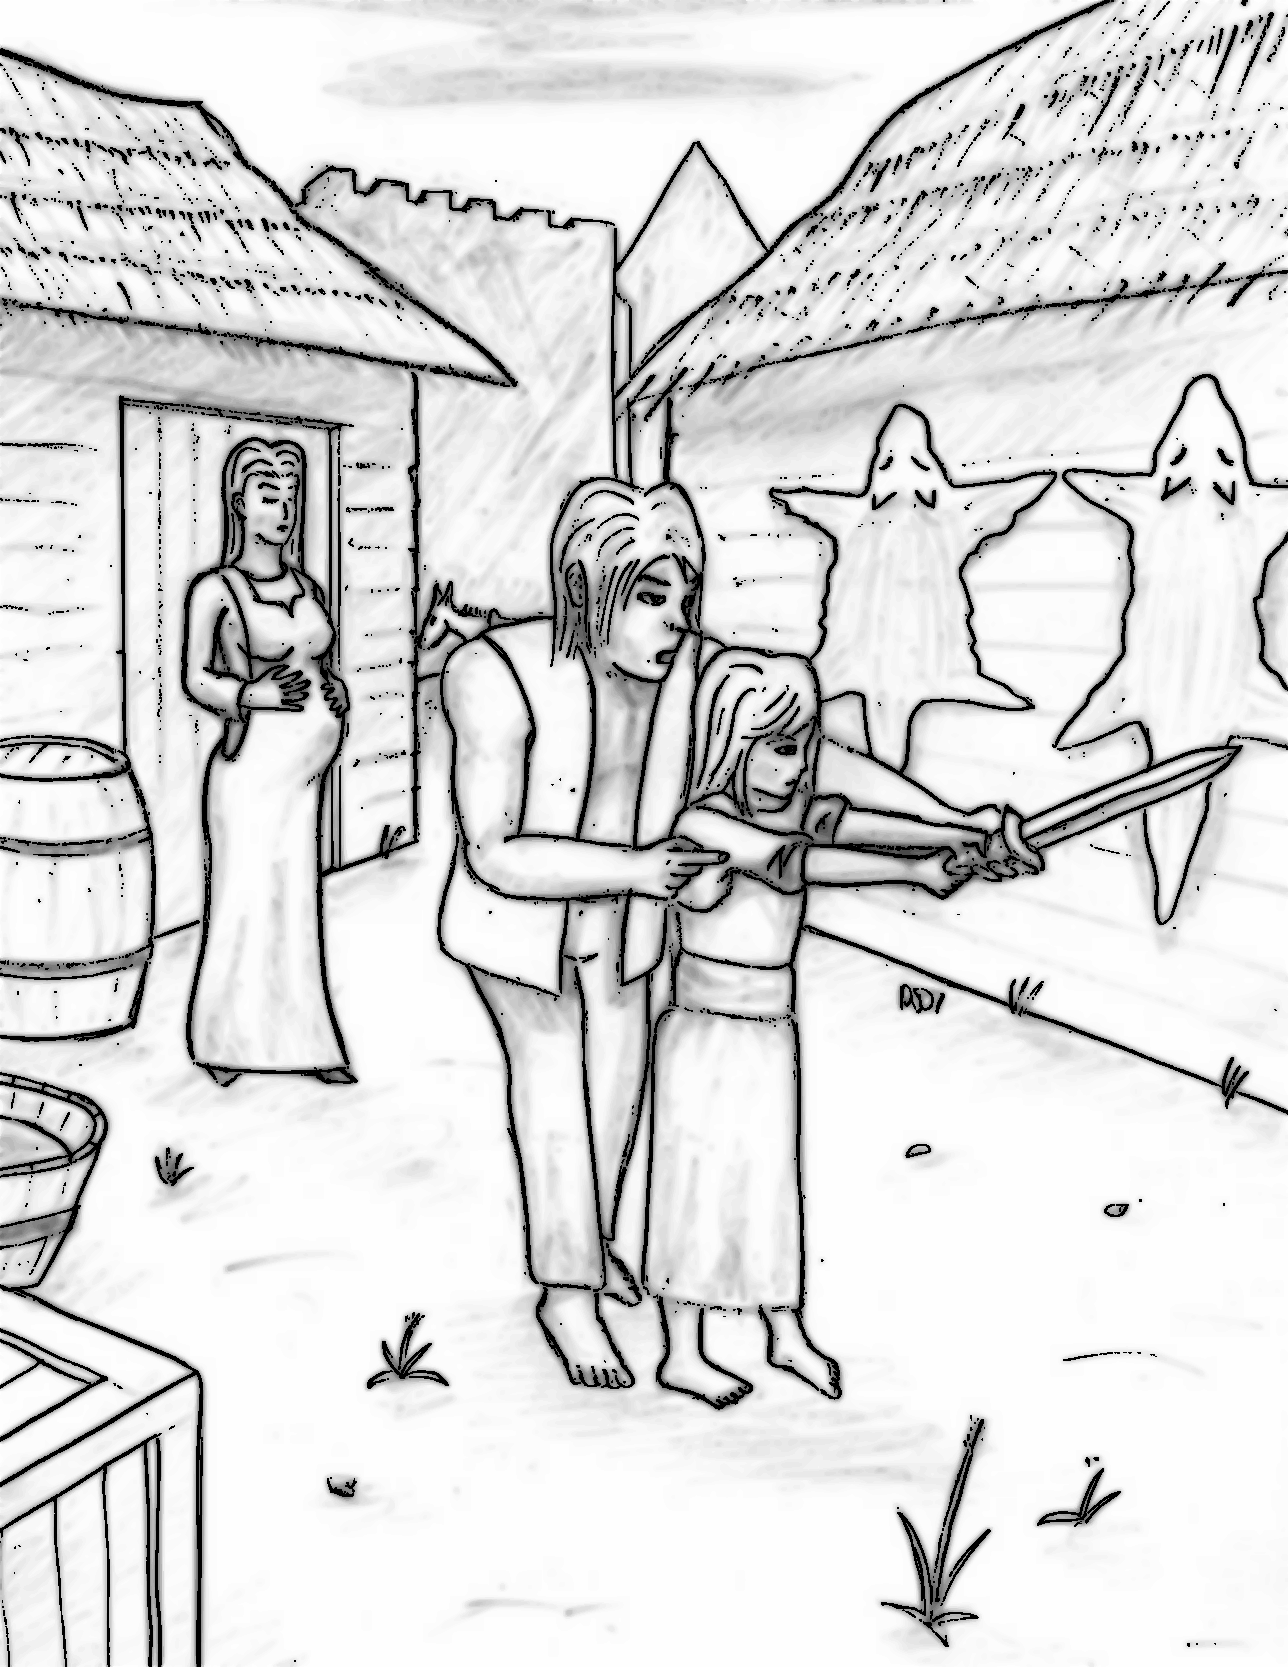
\includepdf[scale=1.007]{instruction.pdf}

